\chapter{Der Touchscreen}
Der Touchscreen von Shulker kann grundsätzlich jeder Touchscreen mit akzeptabler Größe sein.
Die Steuerung des Touchscreens wird von Shulker-Core mithilfe des crates \textbf{slint} (Version 0.2) übernommen.

\section{Funktionsweise von slint}
Um mit slint eine grafische Benutzeroberfläche bereitstellen zu können, wird empfohlen, eine slint-Datei erstellen.
In dieser Datei wird mittels der .slint-Sprache eine Benutzeroberfläche beschrieben und programmiert. Diese Datei wird vom 
slint-Compiler in Binärcode umgewandelt. Da die .slint-Datei und der eigentliche Anwendungscode also getrennt sind, muss man sich
mittels Callbacks, Models und Eigenschaften verständigen. 
\begin{figure}[H]
    \begin{center}
        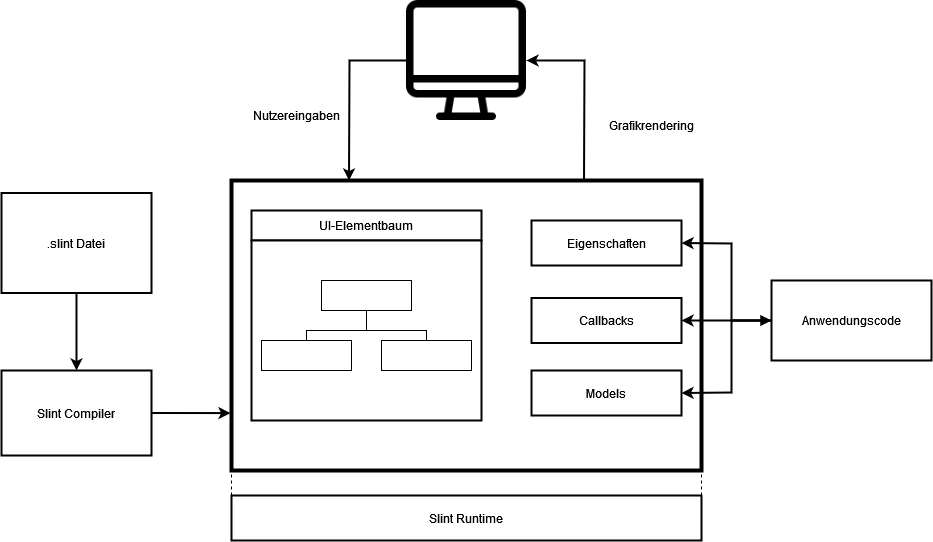
\includegraphics[width=0.9\textwidth]{images/core/slint_aufbau.png}
        \caption{Aufbau und Funktionsweise von slint}
    \end{center}
\end{figure}

\section{Aufbau der grafischen Oberfläche}
Shulker-Core verwendet eine .slint-Datei, welche den Namen \textit{mainwindow.slint} trägt. Diese Datei befindet sich im Unterordner
namens \textit{ui} in der Git-Repository von Shulker. Das Design der Oberfläche konzentriert sich darauf, möglichst leicht
lesbar und stromsparend zu sein. Deshalb entschieden wir uns für die Farben Schwarz und Weiß.

Die grafische Oberfläche besteht aus drei Teilen:
\begin{itemize}
    \item Menü-Selektor
    \item Hauptsicht
    \item Unlocked-Ansicht
\end{itemize}

\subsection{Menü-Selektor}
Der Menü-Selektor ist grundsätzlich immer zu sehen. Die einzige Ausnahme bildet das Entsperrtsein des elektronischen
Schlosses. Der Menü-Selektor ermöglicht das Wechseln der Hauptansicht. Es gibt drei Wahlmöglichkeiten:
\begin{itemize}
    \item \textbf{Pin}: zur Eingabe von Ziffernpins
    \item \textbf{PW}: zur Eingabe von Passwörtern, also Pins mit Buchstaben
    \item \textbf{M}: zur Verbindung mit Shulker-Mobile
\end{itemize}

\subsection{Hauptansicht}
Die Hauptansicht nimmt den Großteil des Bildschirms in Anspruch. In ihr wird dem Nutzer das Eingeben von Pins und Passwörtern
ermöglicht. Ein QR-Code zur Verbindung mit Shulker-Mobile lässt sich auch anzeigen.

\subsection{Unlocked-Ansicht}
Die Unlocked-Ansicht zeigt dem Nutzer, dass das Schloss momentan offen ist. Sie nimmt den ganzen Bildschirm in Anspruch und weicht
als einzige Komponente vom standart Farbschema ab; grelles Grün vermittelt ein klares Signal. Auf ihr ist auch ersichtlich,
wie lange das Schloss noch offen bleibt. Die Ansicht kann über mehrere Wege in den Vordergrund geschoben werden, grundsätzlich aber dann,
wenn an Shulker-Core ein Öffnen-Signal oder ein korrekter Pin gesendet wurde.
